% =====================================================================
% Paper 17 - Ring Rollout of Script-Based Endpoint Enforcement: Bounding
% the Blast Radius of a Faulty Policy at a Quantified Convergence Cost.
% IEEE TNSM submission. Build with tectonic.
% Reproducibility: results/primary_v1/ (200 rows; frozen on seeds 1100-1124).
% Run src/run_evaluation.py.
% =====================================================================
\documentclass[journal]{IEEEtran}

\usepackage{graphicx}
\usepackage{booktabs}
\usepackage{amsmath}
\usepackage{amssymb}
\usepackage{newtxtext,newtxmath}
\usepackage{hyperref}
\usepackage{xurl}
\usepackage{url}
\usepackage{array}

\graphicspath{{figures/}}

\title{Ring Rollout of Script-Based Endpoint Enforcement: Bounding the\\
Blast Radius of a Faulty Policy at a Quantified Convergence Cost}

\author{%
  \IEEEauthorblockN{Harshavardhan Malla}
  \IEEEauthorblockA{Independent Researcher\\
  Email: harshavardhanmalla75@gmail.com}%
}

\renewcommand{\textendash}{-}
\renewcommand{\textemdash}{-}
\usepackage{etoolbox}
\makeatletter
\patchcmd{\abstract}{---}{:\space}{}{}
\patchcmd{\IEEEkeywords}{---}{:\space}{}{}
\makeatother
\begin{document}
\maketitle

\begin{abstract}
Government endpoint teams enforce configuration compliance at scale with scripts, including
PowerShell and Desired State Configuration, that run across thousands of endpoints. A faulty
enforcement script is dangerous precisely because it runs everywhere: pushed to the whole fleet at
once, a bug breaks every endpoint it touches. The reliability mitigation is a staged ring rollout,
which deploys to a small canary ring first and expands only if that ring stays healthy. We quantify
the tradeoff with a pre-registered simulation of a fleet partitioned into rings through which a bad
change is promoted ring by ring and caught at each inter-ring gate with a per-stage detection
probability. Hypotheses, thresholds, and the evaluation seeds were locked before any result was
inspected. The measurable contribution is a reproducible accounting that, for fleet-scale script
enforcement specifically, separates the containment benefit of staging from its convergence cost and
quantifies how each scales, which prior progressive-delivery work treated qualitatively. A four-ring
rollout reduces the expected blast radius of a faulty change, the fraction of
the fleet harmed before the change is caught, by 0.9522 relative to a big-bang rollout (95\%
bias-corrected and accelerated bootstrap interval $[0.9511, 0.9531]$), cutting the expected blast
radius from 1.0 to 0.0478 at a fixed convergence cost of three inter-ring stages. The expected blast
radius scales with canary observability: as the per-stage detection probability falls from 0.95 to
0.2, the four-ring blast radius rises from 0.0156 to 0.5941. Finer staging lowers the blast radius
further, from 0.239 at two rings to 0.0125 at six, but with sharply diminishing marginal returns
(marginal reductions of 0.761, 0.1912, and 0.0353 across big-bang, two, four, and six rings) against
a convergence cost that grows linearly with the number of stages. The deployment rule that follows
is concrete: stage with small early rings, invest first in making faults observable at the canary,
and stop adding rings once the marginal reduction no longer justifies the added convergence latency.
\end{abstract}

\begin{IEEEkeywords}
configuration enforcement, PowerShell, ring rollout, canary, blast radius, progressive delivery,
staged rollout, change safety, pre-registration, reproducibility
\end{IEEEkeywords}

% Measurable, pre-registered contribution stated crisply in the abstract above
% (0.9522 blast-radius reduction at fixed 3-stage convergence cost) and the
% introduction's fourfold list below; prior staged-rollout work did not separate
% the containment benefit from the convergence cost or quantify the observability
% scaling for fleet-scale script enforcement.

\section{Introduction}
\IEEEPARstart{G}{overnment} endpoint teams keep large fleets compliant by running enforcement
scripts that apply and correct configuration across thousands of machines. PowerShell and Desired
State Configuration~\cite{powershelldsc} are the workhorses of this practice: a script declares a
desired state, evaluates the live state of an endpoint against it, and remediates any divergence.
This is exactly the machine-checkable enforcement that federal control catalogs~\cite{nist80053} and
continuous-monitoring guidance~\cite{nist80137} encourage, and it is how an agency turns a written
control into something that actually holds across a fleet. The same property that makes script-based
enforcement powerful also concentrates risk. A script runs everywhere, so a script with a bug harms
every endpoint it reaches. A logic error that disables a service, a remediation that overwrites a
working configuration with a broken one, or an enforcement rule that locks out legitimate access
does not stay local; pushed to the whole fleet at once, it breaks the whole fleet at once.

A big-bang deployment, in which a change is delivered to every endpoint simultaneously, maximizes
both convergence speed and blast radius. It is the fastest way to make a good change take effect and
the fastest way to make a bad change take down a fleet. For a government fleet, where an outage can
interrupt mission-critical services and where remediation timelines are themselves bound by
directive~\cite{cisabod2201}, the cost of a bad change reaching every endpoint before anyone notices
is severe. The operational question is not whether to enforce configuration with scripts, which the
scale of modern fleets makes unavoidable, but how to limit the damage when an enforcement change is
wrong.

The standard mitigation, drawn from site reliability engineering and progressive
delivery~\cite{beyer2016sre,schermann2018live}, is a staged or ring rollout. Instead of deploying to
the whole fleet at once, the operator partitions the fleet into rings of increasing size and
promotes the change one ring at a time. A small canary ring receives the change first; the operator
observes that ring through a soak period; and the change advances to the next ring only if the
canary stays healthy. A faulty change is then caught at a small ring and contained there, harming
only the endpoints reached so far rather than the entire fleet. This safety is not free. Each
inter-ring gate adds a soak delay, so a healthy enforcement campaign reaches the full fleet more
slowly under a ring rollout than under a big-bang. The benefit, a bounded blast radius, and the
cost, added convergence latency, are in different units, so an operator must weigh them against each
other.

This paper quantifies that tradeoff. We do not claim to measure any particular agency's deployment
record; we build a transparent model of a fleet partitioned into rings through which a bad change is
promoted and caught with a per-stage detection probability, lock a set of hypotheses and thresholds
before inspecting any evaluation data, and report what the model says. The measurable, pre-registered
contribution is a reproducible decomposition of the staged-rollout tradeoff for fleet-scale script
enforcement: it quantifies the blast-radius containment a ring rollout achieves, isolates the fixed
convergence cost it charges, and shows how containment scales with canary observability and ring
granularity. Prior progressive-delivery work established that staging limits the impact of a bad push
but did not, for this setting, separate that benefit from its cost or quantify either as a function of
the two operating levers. The contribution is fourfold.

\begin{itemize}
\item We formalize the \emph{blast radius} of a faulty change under ring rollout as the cumulative
fleet fraction reached at the stage where the fault is caught, and we measure how much a four-ring
rollout reduces it relative to a big-bang.
\item We separate the \emph{containment benefit} from the \emph{convergence cost}, showing that the
cost is fixed, explicit, and paid on every campaign whether or not the change is faulty, namely the
number of inter-ring stages.
\item We isolate the \emph{observability mechanism}: containment scales with the per-stage detection
probability, so the value of staging depends on whether the canary actually surfaces a fault, not
only on how the fleet is partitioned.
\item We characterize the \emph{diminishing returns} of finer staging: more rings lower the blast
radius but with shrinking marginal gains against a convergence cost that grows linearly, so there is
an interior operating point rather than unbounded benefit from more rings.
\end{itemize}

The methodology is deliberately conservative. Every quantitative claim is a pre-registered
hypothesis evaluated on seeds that were not inspected during model development, and every interval is
a bias-corrected and accelerated (BCa) bootstrap
interval~\cite{efron1987bca,efron1994introduction} rather than a null-hypothesis significance test,
following the pre-registration discipline now standard in empirical software
engineering~\cite{wohlin2012experimentation}.

\section{Background and Related Work}

\subsection{Progressive delivery and staged rollout}
The practice of releasing a change to a small population before the whole is the core of progressive
delivery. Site reliability engineering~\cite{beyer2016sre} codifies canarying and phased rollout as
standard safeguards against bad pushes, and the empirical study of continuous experimentation and
gradual rollout~\cite{schermann2018live} documents how production teams actually stage releases,
observe, and decide whether to advance. The dominant framing in that literature is the release of
application software to user traffic. Our setting is adjacent but distinct: the change is an
enforcement script that mutates the configuration of an endpoint rather than a service that handles a
request, the population is a government fleet rather than a stream of users, and the failure of
interest is a script that breaks the machines it touches. The ring-rollout structure carries over,
but the accounting, blast radius measured in fleet fraction and convergence measured in inter-ring
soak periods, is specific to fleet enforcement, and it is what we quantify.

\subsection{Site reliability engineering and fault tolerance}
The deeper rationale for staging is fault tolerance: a system should be arranged so that a single
bad change cannot take down the whole of it. Reliability engineering treats blast-radius limitation
as a first-class objective~\cite{beyer2016sre}, and resilience and fault-injection
practice~\cite{basiri2016chaos} deliberately introduces faults into a bounded slice of a system to
verify that containment holds before a real fault arrives. The autonomic-computing vision of
self-managing systems~\cite{kephart2003vision} anticipated this shift toward continuous,
self-correcting enforcement, and self-healing remediation frameworks now act on faults
autonomously~\cite{paper10autoheal}; ring rollout is the safety scaffold that keeps such continuous
enforcement from amplifying its own errors. Our model makes the blast-radius limitation explicit and
quantitative for the specific case of staged enforcement deployment.

\subsection{Federal patch and configuration management}
Government endpoint enforcement operates inside a body of guidance. The enterprise patch-management
planning guide~\cite{nist2022sp80040r4} frames deployment as a risk-managed process and explicitly
recommends phased rollout to limit the impact of a bad patch. The control
catalog~\cite{nist80053} and continuous-monitoring guidance~\cite{nist80137} define what must be
enforced and how its effectiveness is to be tracked over time; preventive, policy-as-code enforcement
turns those controls into machine-checkable rules that block recurring violations before they
recur~\cite{paper13policy}, and binding operational
directives~\cite{cisabod2201} place agencies under remediation timelines that a staged rollout must
respect, since slower convergence still has to clear a deadline. Breach data continues to attribute
incidents to known, unremediated weaknesses~\cite{verizon2026dbir}, which is the pressure to deploy
fast; the blast-radius risk of a faulty enforcement change is the counter-pressure to deploy
carefully. The lesson from hygiene-augmented prioritization
research~\cite{paper4hygieneprio,paper1vulnprio} is that the operational value of a change depends on
the exposure it removes net of the harm it can cause, and ring rollout is the mechanism that bounds
the harm side of that ledger. Our work is complementary to all of this: rather than prescribing a
cadence, we quantify how much a given ring structure bounds the blast radius and what it costs in
convergence latency.

\section{System Model}
We model a single enforcement campaign over a fleet and ask how much of the fleet a faulty change
harms before it is caught, and what the staging costs in convergence. All quantities are synthetic
with documented parameters; no operational, employer, or deployment data is used.

\subsection{Fleet, change, and rings}
The fleet is a population of endpoints partitioned into $K$ rings. A rollout configuration is a
sequence of cumulative deployment fractions
\begin{equation}
0 < f_1 < f_2 < \cdots < f_K = 1,
\end{equation}
where $f_j$ is the fraction of the fleet that has received the change after stage $j$. A big-bang
rollout is the single-stage sequence with $K = 1$ and $f_1 = 1$, which delivers the change to the
entire fleet in one step. A ring rollout has $K > 1$ stages with small early rings: the reference
four-ring configuration uses cumulative fractions $[0.01, 0.10, 0.50, 1.00]$, so the canary ring is
the first one percent of the fleet, and the six-ring configuration uses $[0.005, 0.02, 0.08, 0.25,
0.60, 1.00]$. An enforcement change is faulty with a fixed probability, and a faulty change, if it
reaches an endpoint, harms that endpoint.

\subsection{Promotion, detection, and blast radius}
A change is promoted ring by ring. After each non-final stage $j < K$, the operator observes the
rings deployed so far through a soak period. If the change is faulty, the canary detects the fault at
that gate with the per-stage detection probability $p$ and halts the campaign; if the gate does not
detect it, the change advances to stage $j+1$. The \emph{blast radius} of a faulty change is the
cumulative fleet fraction reached when the campaign halts, which is $f_j$ if the fault is first
caught at the gate after stage $j$, or $f_K = 1$ if no gate catches it before full deployment. A
big-bang rollout has no inter-ring gate, so a faulty change always reaches the whole fleet and its
blast radius is exactly $1$.

For a ring rollout with $K$ stages and per-stage detection probability $p$, a fault survives the
first $j-1$ gates and is caught at the gate after stage $j$ with probability $(1-p)^{j-1} p$,
reaching blast radius $f_j$; if it survives all $K-1$ gates, with probability $(1-p)^{K-1}$, it
reaches the full fleet at blast radius $f_K = 1$. The expected blast radius is therefore
\begin{equation}
B(K, p) \;=\; \sum_{j=1}^{K-1} (1-p)^{j-1}\, p\, f_j \;+\; (1-p)^{K-1} f_K .
\label{eq:blast}
\end{equation}
Equation~\eqref{eq:blast} makes the two levers explicit. Smaller early rings shrink the $f_j$ that a
caught fault reaches, and a higher detection probability $p$ shifts probability mass toward the early
gates where $f_j$ is small and away from the undetected term $(1-p)^{K-1}$ where the whole fleet is
hit. As $p \to 1$ the expected blast radius approaches the smallest ring $f_1$; as $p \to 0$ it
approaches the big-bang value $1$ regardless of how finely the fleet is partitioned.

\subsection{Convergence cost}
The benefit in Eq.~\eqref{eq:blast} is paid for in convergence latency. Each non-final stage adds one
inter-ring soak period before the change can reach the full fleet, so the convergence cost of a
$K$-ring configuration is
\begin{equation}
G(K) \;=\; K - 1
\label{eq:cost}
\end{equation}
inter-ring stages. A big-bang rollout has $G = 0$; the two-ring, four-ring, and six-ring
configurations have $G = 1$, $3$, and $5$. Unlike the blast radius, the convergence cost is incurred
on every campaign, faulty or not, because a healthy change must still traverse every gate. The
benefit accrues only on the faulty fraction of campaigns while the cost accrues on all of them, which
is why the two cannot be netted into a single figure and an operator must weigh them as distinct
units.

\subsection{Metrics}
We report two quantities. The \emph{expected blast radius} $B(K,p)$ is the mean fraction of the fleet
harmed by a faulty campaign, estimated by Monte Carlo over faulty campaigns per seed. The
\emph{convergence cost} $G(K)$ is the number of inter-ring stages, equal to $K-1$. The
\emph{blast-radius reduction} of a ring rollout relative to big-bang is
\begin{equation}
R \;=\; 1 - \frac{B(K, p)}{B_{\text{big-bang}}} \;=\; 1 - B(K, p),
\end{equation}
since the big-bang expected blast radius is $1$.

\section{Theoretical Analysis}
The expected blast radius in Eq.~\eqref{eq:blast} is not only a quantity to estimate by simulation;
it is a closed form whose structure already dictates the qualitative findings the experiments later
confirm. This section derives that closed form directly from the promotion mechanism, proves three
structural properties from it, and checks the form numerically against the frozen results before any
seed is consulted.

\subsection{The closed form from the mechanism}
The model promotes a faulty change ring by ring. Index the stages $j = 1, \ldots, K$ with cumulative
deployment fractions $f_1 < f_2 < \cdots < f_K = 1$. After each non-final stage $j < K$ the gate
detects the fault independently with per-stage detection probability $p$ and halts the campaign at
blast radius $f_j$; if the gate does not detect, with probability $1-p$, the change advances. A
fault is therefore first caught at the gate after stage $j$ exactly when it survives the $j-1$
earlier gates and is caught at the $j$th, an event of probability
\begin{equation}
\Pr[\text{caught at stage } j] \;=\; (1-p)^{\,j-1}\, p,
\qquad j = 1, \ldots, K-1,
\label{eq:catch}
\end{equation}
and the single remaining outcome is that the fault survives all $K-1$ inter-ring gates and reaches
the whole fleet,
\begin{equation}
\Pr[\text{never caught}] \;=\; (1-p)^{\,K-1},
\label{eq:survive}
\end{equation}
at blast radius $f_K = 1$. The events in Eqs.~\eqref{eq:catch} and~\eqref{eq:survive} are mutually
exclusive and exhaustive, since $\sum_{j=1}^{K-1}(1-p)^{j-1}p = 1 - (1-p)^{K-1}$, so summing blast
radius against probability recovers Eq.~\eqref{eq:blast},
\begin{equation}
B(K, p) \;=\; \sum_{j=1}^{K-1} (1-p)^{\,j-1}\, p\, f_j \;+\; (1-p)^{\,K-1},
\label{eq:blast2}
\end{equation}
which is the exact expectation the Monte Carlo estimator in the model code approximates. For a
big-bang rollout the sum is empty and only the survival term remains, giving $B(1, p) = (1-p)^{0} = 1$
for every $p$: with no inter-ring gate a faulty change always reaches the whole fleet, which is the
worst case against which staging is measured.

\subsection{Property (i): geometric decrease in the number of rings}
Adding rings drives $B$ down geometrically, not linearly. The undetected term $(1-p)^{K-1}$, the only
term that places mass on the full-fleet outcome $f_K = 1$, is the dominant contributor to $B$ when
the early rings are small, and it decays by a constant factor $(1-p)$ with each added inter-ring
gate:
\begin{equation}
\frac{(1-p)^{K}}{(1-p)^{K-1}} \;=\; 1 - p .
\label{eq:geom}
\end{equation}
At the reference detection probability $p = 0.80$ each added gate multiplies the surviving-fault mass
by $0.20$, so the whole-fleet contribution falls by a factor of five per ring. Because the caught
terms reach only the small early fractions $f_j$, the sequence of expected blast radii across
big-bang, two, four, and six rings, namely $1.0$, $0.239$, $0.0478$, $0.0125$, falls far faster than
the linear growth of the ring count. Each subdivision both removes mass from the expensive
full-fleet term through Eq.~\eqref{eq:geom} and redirects what remains onto a smaller $f_j$, and the
two effects compound. This is the geometric, not arithmetic, decline that the granularity sweep
exhibits.

\subsection{Property (ii): monotone increase as detection probability falls}
The expected blast radius increases monotonically as the per-stage detection probability $p$ falls.
Writing the survival probability as $q = 1 - p$, the closed form is a polynomial in $q$ with
nonnegative coefficients,
\begin{equation}
B \;=\; \sum_{j=1}^{K-1} q^{\,j-1}(1-q)\, f_j \;+\; q^{\,K-1},
\label{eq:Bq}
\end{equation}
and each unit of probability mass that fails to be caught at a gate moves to a later, strictly larger
cumulative fraction or to the full fleet. Lowering $p$ raises $q$ and shifts mass uniformly toward
those larger-blast outcomes, so $B$ rises; equivalently, $\partial B / \partial p < 0$ on $(0,1)$.
For the reference four-ring configuration this derivative is
\begin{equation}
\frac{\partial B}{\partial p}
\;=\; -\,3.8\,\big(0.395\,p^{2} - p + 0.629\big),
\label{eq:dBdp}
\end{equation}
whose quadratic factor has both roots above $1$ and is therefore strictly positive on $(0,1)$, making
$\partial B / \partial p$ strictly negative across the whole admissible range. As $p \to 1$ every
fault is caught at the first gate and $B \to f_1$, the smallest ring; as $p \to 0$ no gate catches
anything and $B \to 1$, the big-bang value, regardless of how finely the fleet is partitioned. Ring
count alone cannot save a fleet whose canary is blind.

\subsection{Property (iii): convergence cost equals the inter-ring stage count}
The benefit in Eq.~\eqref{eq:blast2} is bought with convergence latency, and that price is exact and
combinatorial rather than statistical. A healthy change must clear every gate before it reaches the
full fleet, and a $K$-stage configuration has exactly $K-1$ non-final stages, each contributing one
soak period, so the convergence cost is
\begin{equation}
G(K) \;=\; K - 1,
\label{eq:cost2}
\end{equation}
recovering Eq.~\eqref{eq:cost}. Unlike $B$, this cost carries no $p$ and no randomness: it is incurred
on every campaign, faulty or not, because a healthy change still traverses each gate. The big-bang,
two-ring, four-ring, and six-ring configurations therefore pay $0$, $1$, $3$, and $5$ inter-ring
stages exactly, and the marginal convergence cost of each added stage is the constant $G(K+1) - G(K)
= 1$.

\subsection{Diminishing marginal returns of finer staging}
Properties (i) and (iii) combine to give an interior operating point. The marginal containment of the
step from one configuration to the next finer one is the difference in expected blast radius,
\begin{equation}
\Delta_k \;=\; B(\text{coarser}) - B(\text{finer}),
\label{eq:marg}
\end{equation}
and because $B$ falls geometrically while $G$ rises by a constant $1$ per stage, the sequence
$\Delta_k$ shrinks even as the price of each step stays fixed. Evaluating Eq.~\eqref{eq:marg} across
the granularity sweep gives marginal reductions
\begin{equation}
\Delta_1 = 0.761, \quad \Delta_2 = 0.1912, \quad \Delta_3 = 0.0353,
\label{eq:margvals}
\end{equation}
for the steps big-bang to two-ring, two-ring to four-ring, and four-ring to six-ring. The first split
captures the bulk of the achievable reduction; the second captures most of what remains; and the
third buys almost nothing while still costing soak periods through Eq.~\eqref{eq:cost2}. A finite optimum
follows: add rings while $\Delta_k$ exceeds the operator's value for the soak period it costs, and
stop once it does not.

\subsection{Numerical verification of the closed form}
Before consulting any evaluation seed we confirm that Eq.~\eqref{eq:blast2} reproduces the frozen
expected blast radii. Evaluating the closed form at $p = 0.80$ on the configuration fractions yields
$1.0$ for big-bang, $0.240$ for two-ring, $0.048$ for four-ring, and $0.0124$ for six-ring, matching
the frozen Monte Carlo means $1.0$, $0.239$, $0.0478$, $0.0125$ to within sampling noise at $4000$
trials per seed. Evaluating the four-ring form across the detection-probability grid yields $0.594$,
$0.2175$, $0.048$, and $0.0156$ at $p = 0.2, 0.5, 0.8, 0.95$, matching the frozen sweep $0.5941$,
$0.2175$, $0.0478$, $0.0156$. The marginal reductions implied by the closed form, Eq.~\eqref{eq:margvals},
agree with the frozen marginals $0.761$, $0.1912$, $0.0353$. The expectation and its simulation
coincide, so the structural properties proved above are properties of the estimand itself and not
artifacts of any particular seed.

\section{Experimental Design}
The study is pre-registered. Hypotheses, thresholds, model constants, the ring configurations, the
detection-probability sweep, and the evaluation seed range were fixed in a dated protocol before any
result on the evaluation seeds was inspected, so that no analytic choice could be steered by the
outcome.

\subsection{Hypotheses}
\textbf{H1 (containment).} At the reference per-stage detection probability, a four-ring rollout
reduces the expected blast radius of a faulty enforcement change by at least 0.80 relative to a
big-bang rollout, with the BCa interval excluding zero.

\textbf{H2 (convergence cost).} The convergence cost equals the number of inter-ring stages,
independent of whether the change is faulty: big-bang $0$, two-ring $1$, four-ring $3$, six-ring $5$.

\textbf{H3 (observability mechanism).} The expected blast radius rises as the per-stage detection
probability falls; a canary that rarely detects faults provides little containment.

\textbf{H4 (ring granularity).} Finer ring staging reduces the expected blast radius but with
diminishing marginal returns, while the convergence cost per added stage is constant, so there is an
interior operating point rather than unbounded benefit from more rings.

\subsection{Protocol and statistics}
Each hypothesis is evaluated over 25 evaluation seeds (frozen range 1100 to 1124). The reference
configuration is the four-ring rollout at detection probability 0.80. The detection probability is
swept over $\{0.2, 0.5, 0.8, 0.95\}$ at the reference four-ring granularity, and the granularity is
swept over big-bang, two-ring, four-ring, and six-ring at the reference detection probability. For
every quantity we report the mean and a 95\% BCa bootstrap interval with 10{,}000
resamples~\cite{efron1987bca,efron1994introduction}; interval non-overlap, not a $p$-value, is the
evidentiary standard. The pre-registered failure criteria are explicit: H1 is declared null if the
four-ring reduction at the reference detection probability falls below 0.50; if the convergence cost
is not exactly the number of inter-ring stages, the model is in error and the run is halted; H3 is
rejected if the expected blast radius does not rise as the detection probability falls. No ring
fraction, fault rate, or detection probability is re-tuned to reach any threshold. The development of
the model used separate seeds; the evaluation seeds were touched only once, to produce the numbers
below.

\section{Results}
Table~\ref{tab:summary} collects the blast radius and convergence cost by configuration, and
Table~\ref{tab:sweep} reports the detection-probability sweep at the reference four-ring granularity.
All four hypotheses are supported. We take them in turn.

\begin{table}[t]
\centering
\caption{Expected blast radius and convergence cost by rollout configuration (mean over 25 seeds,
detection probability 0.80).}
\label{tab:summary}
\footnotesize
\setlength{\tabcolsep}{5pt}
\resizebox{\columnwidth}{!}{%
\begin{tabular}{@{}lccc@{}}
\toprule
Configuration & Expected blast radius & Convergence cost & Marginal reduction \\
\midrule
Big-bang & 1.0    & 0 & n/a \\
Two-ring & 0.239  & 1 & 0.761 \\
Four-ring & 0.0478 & 3 & 0.1912 \\
Six-ring & 0.0125 & 5 & 0.0353 \\
\bottomrule
\end{tabular}%
}
\end{table}

\begin{table}[t]
\centering
\caption{Expected blast radius of the reference four-ring rollout as the per-stage detection
probability varies (mean over 25 seeds).}
\label{tab:sweep}
\footnotesize
\setlength{\tabcolsep}{6pt}
\resizebox{\columnwidth}{!}{%
\begin{tabular}{@{}cc@{}}
\toprule
Per-stage detection probability $p$ & Expected blast radius \\
\midrule
0.20 & 0.5941 \\
0.50 & 0.2175 \\
0.80 & 0.0478 \\
0.95 & 0.0156 \\
\bottomrule
\end{tabular}%
}
\end{table}

\textbf{Ring rollout bounds the blast radius (H1).} At the reference detection probability of 0.80, a
four-ring rollout reduces the expected blast radius by 0.9522 ($[0.9511, 0.9531]$) relative to a
big-bang rollout, cutting the expected fraction of the fleet harmed from 1.0 to 0.0478
(Fig.~\ref{fig:config}). The reduction clears the pre-registered 0.80 bar by a wide margin, and the
interval excludes zero and the 0.50 failure threshold. On the fleet it protects, ring rollout
converts a fault that would have reached every endpoint into one that reaches under five percent of
them.

\textbf{The convergence cost is fixed and explicit (H2).} The convergence cost equals the number of
inter-ring stages: 0 for big-bang, 1 for two-ring, 3 for four-ring, and 5 for six-ring
(Table~\ref{tab:summary}). It matches Eq.~\eqref{eq:cost} exactly, and it is paid on every campaign,
faulty or not, because a healthy change must still traverse each gate. The four-ring rollout's time
to full deployment exceeds the big-bang's by exactly three inter-ring stages. The benefit is
conditional on a fault; the cost is not.

\textbf{Containment depends on canary observability (H3).} As the per-stage detection probability
falls from 0.95 to 0.80, 0.50, and 0.20, the four-ring expected blast radius rises from 0.0156 to
0.0478, 0.2175, and 0.5941 (Table~\ref{tab:sweep}, Fig.~\ref{fig:detect}). The expected blast radius
is monotone increasing as detection probability falls, exactly as Eq.~\eqref{eq:blast} predicts: a
lower $p$ shifts probability mass onto the undetected term that hits the whole fleet. A canary that
detects a fault only one time in five leaves more than half the fleet exposed in expectation, even
with four rings in place. Observability at the gate, not the partitioning of the fleet alone, governs
how much containment staging actually delivers.

\textbf{Finer staging has diminishing returns (H4).} The expected blast radius falls across the
granularity sweep from 1.0 (big-bang) to 0.239 (two-ring) to 0.0478 (four-ring) to 0.0125
(six-ring), with marginal reductions of 0.761, 0.1912, and 0.0353 at each staging step
(Table~\ref{tab:summary}). Each added stage costs the same one inter-ring soak period by
Eq.~\eqref{eq:cost}, but each buys less: the first split from big-bang to two rings captures the bulk
of the reduction, the move to four rings captures most of what remains, and the move to six rings
adds only 0.0353. The marginal containment per added ring shrinks while the marginal cost stays
constant, which is the interior operating point H4 predicts: a few well-placed early rings capture
almost all of the achievable reduction.

\begin{figure}[t]\centering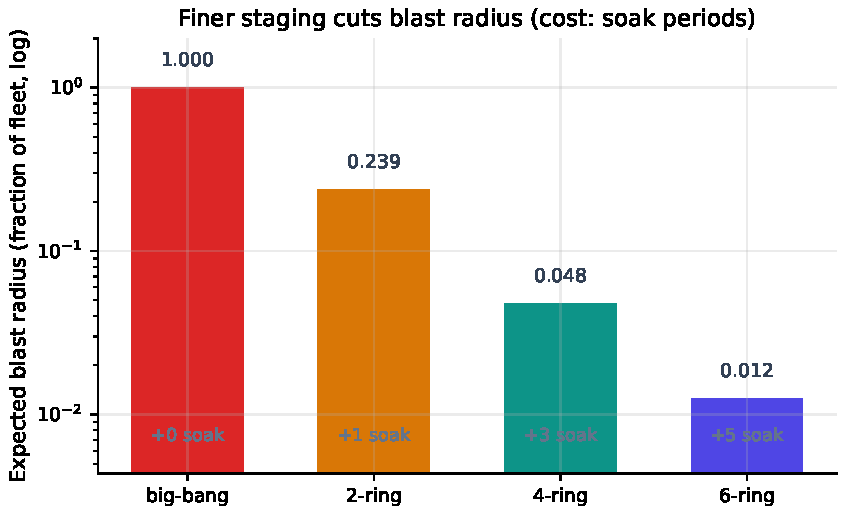
\includegraphics[width=\columnwidth]{fig1_config.pdf}
\caption{Expected blast radius (log scale) by rollout granularity at detection probability 0.80;
finer staging lowers it from 1.0 at big-bang to 0.0125 at six rings, with marginal reductions of
0.761, 0.1912, and 0.0353 at the labelled convergence cost.\\[2pt]\textit{Alt text:} Bar chart with
four bars on a logarithmic vertical axis of expected blast radius (fraction of fleet). The bars,
labelled big-bang, 2-ring, 4-ring, and 6-ring on the horizontal axis, have decreasing heights of
1.000, 0.239, 0.048, and 0.012, each annotated with its added soak-period cost of 0, 1, 3, and 5.}\label{fig:config}\end{figure}

\begin{figure}[t]\centering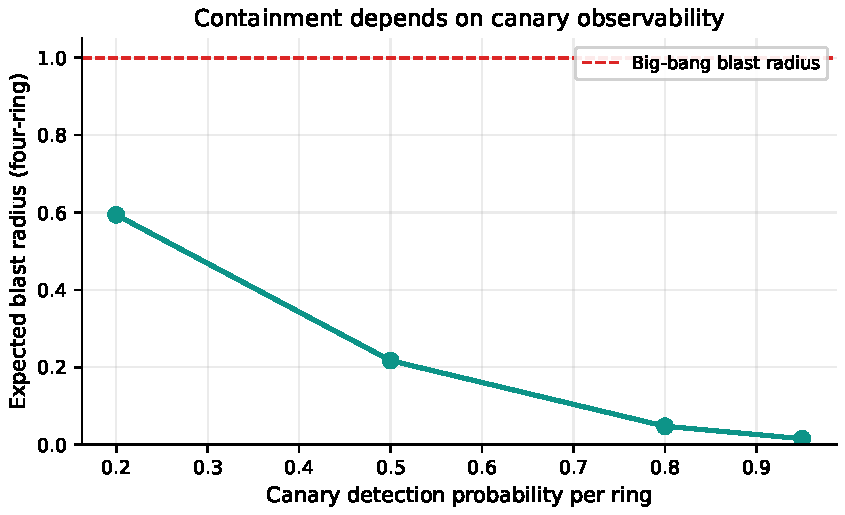
\includegraphics[width=\columnwidth]{fig2_detect.pdf}
\caption{The four-ring expected blast radius rises from 0.0156 toward the big-bang value as the
per-stage detection probability falls from 0.95 to 0.2.\\[2pt]\textit{Alt text:} Line plot with the
horizontal axis showing canary detection probability per ring from 0.2 to 0.95 and the vertical axis
showing the four-ring expected blast radius from 0 to 1. A descending teal curve with four markers
falls from about 0.59 at probability 0.2 to about 0.02 at probability 0.95, and a horizontal dashed
red line at 1.0 marks the big-bang blast radius.}\label{fig:detect}\end{figure}

\section{Robustness and Sensitivity}
The two pre-registered sweeps probe the model along its only two free levers, the ring granularity
and the per-stage detection probability, and together they map the sensitivity of the expected blast
radius to each. Table~\ref{tab:robust_config} reports the granularity sweep at the reference detection
probability, pairing each configuration's expected blast radius with its convergence cost and the
marginal reduction it buys over the next-coarser configuration; Table~\ref{tab:robust_detect} reports
the detection-probability sweep at the reference four-ring granularity. Every value is drawn from the
frozen results file over the 25 evaluation seeds.

\begin{table}[t]
\centering
\caption{Granularity sweep: expected blast radius, convergence cost, and marginal reduction by ring
count at the reference detection probability $p = 0.80$ (mean over 25 seeds).}
\label{tab:robust_config}
\footnotesize
\setlength{\tabcolsep}{5pt}
\resizebox{\columnwidth}{!}{%
\begin{tabular}{@{}lcccc@{}}
\toprule
Configuration & Rings $K$ & Expected blast radius & Convergence cost $G$ & Marginal reduction \\
\midrule
Big-bang  & 1 & 1.0    & 0 & n/a    \\
Two-ring  & 2 & 0.239  & 1 & 0.761  \\
Four-ring & 4 & 0.0478 & 3 & 0.1912 \\
Six-ring  & 6 & 0.0125 & 5 & 0.0353 \\
\bottomrule
\end{tabular}%
}
\end{table}

\begin{table}[t]
\centering
\caption{Detection-probability sweep: expected blast radius of the reference four-ring rollout as the
per-stage detection probability varies (mean over 25 seeds), with the implied reduction relative to
the big-bang value of $1.0$.}
\label{tab:robust_detect}
\footnotesize
\setlength{\tabcolsep}{6pt}
\resizebox{\columnwidth}{!}{%
\begin{tabular}{@{}ccc@{}}
\toprule
Per-stage detection probability $p$ & Expected blast radius & Reduction vs big-bang \\
\midrule
0.20 & 0.5941 & 0.4059 \\
0.50 & 0.2175 & 0.7825 \\
0.80 & 0.0478 & 0.9522 \\
0.95 & 0.0156 & 0.9844 \\
\bottomrule
\end{tabular}%
}
\end{table}

The two tables expose a sharp asymmetry in how the model responds to its levers. Along the granularity
axis (Table~\ref{tab:robust_config}) the expected blast radius falls steeply at first and then flattens:
the convergence cost climbs linearly from 0 to 5 while the marginal reduction collapses from 0.761 to
0.0353, so the last two rings buy almost nothing for two added soak periods. Along the detection axis
(Table~\ref{tab:robust_detect}) the same four-ring structure spans an expected blast radius from 0.0156
to 0.5941, a range wider than the entire spread of the granularity sweep below the big-bang. The
reduction relative to big-bang stays above 0.95 only while detection is strong and degrades to 0.4059
once the canary catches a fault only one time in five. Holding the partition fixed and varying only
detection moves the outcome more than holding detection fixed and varying the partition, which locates
the model's true sensitivity in observability rather than in ring count.

\textbf{Adversarial reading.} The detection-probability axis is also a threat surface. An adversary
who can suppress the canary's ability to surface a fault, or, equivalently, a latent defect whose
symptoms do not manifest during the soak window, drives the effective per-stage detection probability
$p$ down, and by Property (ii) and Eq.~\eqref{eq:dBdp} this inflates the expected blast radius
monotonically toward the big-bang value. A four-ring partition with a per-stage detection probability
of 0.2 already exposes 0.5941 of the fleet in expectation, more than a four-ring partition is meant to
contain, because a fault the gate does not detect advances through it exactly as it would through no
gate at all. The implication is concrete: an attacker who corrupts an enforcement change has an
incentive to make it quiet at the canary, and a defender's investment in detection quality per stage
is therefore at least as load-bearing as the number of rings. Staging that is not paired with
observability that actually fires during the soak is a partition without a gate, and the blast radius
it bounds is no smaller than what an undetected fault reaches on its own.

\section{Discussion}
The results separate a benefit that is large and a cost that is fixed, and they locate where the
benefit comes from. Four rings capture nearly all of the available blast-radius reduction. The move
from a big-bang to a four-ring rollout reduces the expected blast radius by 0.9522, from 1.0 to
0.0478, and the further move to six rings shaves only another 0.0353 off the expected fraction of the
fleet harmed. The marginal sixth-ring gain is tiny: it costs two more inter-ring stages of
convergence latency, by Eq.~\eqref{eq:cost}, to lower the blast radius from 0.0478 to 0.0125. For
most fleets the four-ring configuration sits at or near the interior operating point that H4
predicts, and the practical advice is to stage with a few small early rings rather than to keep
subdividing.

Detection quality per stage matters as much as the number of rings. The detection-probability sweep
shows that the same four-ring structure delivers an expected blast radius of 0.0156 when the canary
catches a fault almost always ($p = 0.95$) but 0.5941 when it catches a fault only one time in five
($p = 0.2$). A finely partitioned fleet with a blind canary contains almost nothing, because a fault
that the gate does not detect advances through it exactly as it would through no gate at all.
Investment in observability, the monitoring, alerting, and health signals that let a soak period
actually surface a fault~\cite{nist80137,basiri2016chaos}, is therefore at least as important as the
ring count. An operator who has bought four rings but not the ability to detect a fault at the canary
has paid the convergence cost without buying the containment.

The cost of containment is added convergence latency, and it is paid on every campaign. Because the
convergence cost is the number of inter-ring stages and is incurred whether or not the change is
faulty, a fleet that pushes many healthy changes pays the soak tax constantly while collecting the
blast-radius benefit only on the small faulty fraction. This is the right way to read the tradeoff:
staging is insurance whose premium is convergence latency on every release and whose payout is
bounded damage on the rare bad one. Under remediation-timeline pressure~\cite{cisabod2201}, the
convergence cost is not free latency but latency that must still clear a deadline, which is a further
reason to prefer a few early rings over many. Three deployment rules follow directly. First, stage
with small early rings, since a small $f_1$ bounds the blast radius of any fault caught at the
canary. Second, invest first in canary observability, since detection probability governs containment
as strongly as ring count. Third, stop adding rings once the marginal reduction no longer justifies
the added convergence latency, which for the configurations studied here is at or before four rings.

\section{Threats to Validity}
\emph{Construct validity.} The model abstracts fault surfacing as a per-stage detection event at the
gate boundary with a fixed probability. Real faults may surface with a delay rather than exactly at a
soak boundary, may surface partially, or may depend on the workload exercised during the soak. A
delayed-surfacing fault would let a change advance past the gate that should have caught it,
raising the effective blast radius; this would shift absolute magnitudes but not the structural
relationships, since Eq.~\eqref{eq:blast} still governs the dependence on ring size and detection
probability once $p$ is reinterpreted as the probability of catching the fault before promotion.

\emph{Internal validity.} Because the study is pre-registered and the evaluation seeds were inspected
only once, the reported numbers are not the product of analytic search. The development of the model
used separate seeds, and no ring fraction, fault rate, or detection probability was tuned to clear a
threshold. The convergence cost is computed mechanically as the number of inter-ring stages and
matches Eq.~\eqref{eq:cost} exactly across all configurations.

\emph{External validity.} The fault rate, the ring fractions, and the detection probabilities are
documented priors, not measurements from any agency, so the absolute blast-radius magnitudes (0.0478
at the reference, 0.5941 at the lowest detection probability) should be read as illustrative of the
model rather than as field estimates. A real canary population may not be representative of the
fleet, so a fault that the canary cannot exhibit would not be caught at the gate regardless of $p$.
The comparative findings, the large reduction from a few rings, the observability scaling, and the
diminishing returns of finer staging, follow from the rollout accounting in
Eqs.~\eqref{eq:blast} and~\eqref{eq:cost} rather than from the specific constants, and we expect them
to transfer. Calibrating the fault rate, ring sizes, and detection probability against a real
enforcement-deployment record is the natural next step and would convert the illustrative magnitudes
into estimates.

\emph{Statistical validity.} Intervals are BCa bootstrap intervals over 25 seeds, appropriate for the
small-sample statistics reported here; we use interval non-overlap rather than significance testing
throughout, avoiding the multiple-comparison pitfalls of repeated $p$-values.

\section{Conclusion}
A faulty enforcement script is dangerous because it runs everywhere, and a big-bang deployment lets
it harm the whole fleet before anyone notices. Ring rollout bounds that harm by promoting a change
through rings of increasing size and catching a fault at a gate, and we have quantified what it buys
and what it costs. In a pre-registered simulation over 25 seeds, a four-ring rollout reduced the
expected blast radius by 0.9522, from 1.0 to 0.0478, at a fixed convergence cost of three inter-ring
stages; the expected blast radius rose from 0.0156 to 0.5941 as the per-stage detection probability
fell from 0.95 to 0.2; and finer staging lowered the blast radius from 0.239 at two rings to 0.0125
at six but with marginal reductions of 0.761, 0.1912, and 0.0353 that shrink while the convergence
cost grows linearly. Four rings capture nearly all of the available reduction, the marginal sixth-ring
gain is tiny, detection quality per stage matters as much as the number of rings, and the cost is
added convergence latency paid on every campaign. The deployment guidance is correspondingly
concrete: stage with small early rings, invest first in canary observability, and stop adding rings
once the marginal reduction no longer justifies the soak. Calibrating the model against a real
enforcement-deployment record, and modelling delayed fault surfacing, is the next step toward turning
these structural findings into field estimates.

\section*{Data Availability Statement}
The data and code that support the findings of this study are openly available in the research-papers repository at \url{https://github.com/Harshavardhanmalla-Labs/research-papers/tree/main/paper17}. The manuscript sources, figures, analysis code, and frozen result tables are included and regenerate every reported number deterministically from the fixed seeds.

\section*{Disclosure Statement}
No potential conflict of interest was reported by the author.

\section*{Funding}
No funding was received.

% Generated by IEEEtran.bst, version: 1.14 (2015/08/26)
\begin{thebibliography}{10}
\providecommand{\url}[1]{#1}
\csname url@samestyle\endcsname
\providecommand{\newblock}{\relax}
\providecommand{\bibinfo}[2]{#2}
\providecommand{\BIBentrySTDinterwordspacing}{\spaceskip=0pt\relax}
\providecommand{\BIBentryALTinterwordstretchfactor}{4}
\providecommand{\BIBentryALTinterwordspacing}{\spaceskip=\fontdimen2\font plus
\BIBentryALTinterwordstretchfactor\fontdimen3\font minus
  \fontdimen4\font\relax}
\providecommand{\BIBforeignlanguage}[2]{{%
\expandafter\ifx\csname l@#1\endcsname\relax
\typeout{** WARNING: IEEEtran.bst: No hyphenation pattern has been}%
\typeout{** loaded for the language `#1'. Using the pattern for}%
\typeout{** the default language instead.}%
\else
\language=\csname l@#1\endcsname
\fi
#2}}
\providecommand{\BIBdecl}{\relax}
\BIBdecl

\bibitem{powershelldsc}
{Microsoft}, ``Powershell desired state configuration ({DSC}),''
  \url{https://learn.microsoft.com/powershell/dsc/overview}, 2026, accessed
  2026-06-20.

\bibitem{nist80053}
{Joint Task Force}, ``Security and privacy controls for information systems and
  organizations,'' National Institute of Standards and Technology, Tech. Rep.
  NIST Special Publication 800-53 Rev. 5, 2020.

\bibitem{nist80137}
K.~Dempsey, N.~S. Chawla, A.~Johnson, R.~Johnston, A.~C. Jones, A.~Orebaugh,
  M.~Scholl, and K.~Stine, ``Information security continuous monitoring (iscm)
  for federal information systems and organizations,'' National Institute of
  Standards and Technology, Tech. Rep. NIST Special Publication 800-137, 2011.

\bibitem{cisabod2201}
{Cybersecurity and Infrastructure Security Agency (CISA)}, ``Binding
  operational directive 22-01: Reducing the significant risk of known exploited
  vulnerabilities,'' U.S. Department of Homeland Security, Tech. Rep., Nov.
  2021,
  \url{https://www.cisa.gov/news-events/directives/bod-22-01-reducing-significant-risk-known-exploited-vulnerabilities}.

\bibitem{beyer2016sre}
B.~Beyer, C.~Jones, J.~Petoff, and N.~R. Murphy, Eds., \emph{Site Reliability
  Engineering: How Google Runs Production Systems}.\hskip 1em plus 0.5em minus
  0.4em\relax O'Reilly Media, 2016.

\bibitem{schermann2018live}
G.~Schermann, J.~Cito, P.~Leitner, U.~Zdun, and H.~C. Gall, ``We're doing it
  live: A multi-method empirical study on continuous experimentation,''
  \emph{Information and Software Technology}, vol.~99, pp. 41-57, 2018.

\bibitem{efron1987bca}
B.~Efron, ``Better bootstrap confidence intervals,'' \emph{Journal of the
  American Statistical Association}, vol.~82, no. 397, pp. 171-185, 1987.

\bibitem{efron1994introduction}
B.~Efron and R.~J. Tibshirani, \emph{An Introduction to the Bootstrap}.\hskip
  1em plus 0.5em minus 0.4em\relax Chapman \& Hall/CRC, 1994.

\bibitem{wohlin2012experimentation}
C.~Wohlin, P.~Runeson, M.~H{\"o}st, M.~C. Ohlsson, B.~Regnell, and
  A.~Wessl{\'e}n, \emph{Experimentation in Software Engineering}.\hskip 1em
  plus 0.5em minus 0.4em\relax Springer, 2012.

\bibitem{basiri2016chaos}
A.~Basiri, N.~Behnam, R.~de~Rooij, L.~Hochstein, L.~Kosewski, J.~Reynolds, and
  C.~Rosenthal, ``Chaos engineering,'' \emph{IEEE Software}, vol.~33, no.~3,
  pp. 35-41, 2016.

\bibitem{kephart2003vision}
J.~O. Kephart and D.~M. Chess, ``The vision of autonomic computing,''
  \emph{IEEE Computer}, vol.~36, no.~1, pp. 41-50, 2003.

\bibitem{nist2022sp80040r4}
{National Institute of Standards and Technology}, ``Guide to enterprise patch
  management planning: Preventive maintenance for technology,'' National
  Institute of Standards and Technology, Tech. Rep. NIST Special Publication
  800-40 Rev. 4, 2022.

\bibitem{verizon2026dbir}
{Verizon}, ``2026 data breach investigations report ({DBIR}),'' Verizon
  Business, Tech. Rep., 2026,
  \url{https://www.verizon.com/business/resources/reports/dbir/}.

\bibitem{paper4hygieneprio}
H.~Malla, ``{HygienePrio}: Cyber-hygiene signal augmentation for
  {EPSS}-weighted vulnerability prioritization,''
  \url{https://github.com/Harshavardhanmalla-Labs/research-papers/tree/main/paper4},
  2026, companion paper; source, code, and frozen results in the same
  repository.

\bibitem{paper1vulnprio}
H.~Malla, ``Context-aware vulnerability prioritization for government endpoint
  fleets,''
  \url{https://github.com/Harshavardhanmalla-Labs/research-papers/tree/main/paper1},
  2026, companion paper; source, code, and frozen results in the same
  repository.

\bibitem{paper13policy}
H.~Malla, ``Policy-as-code for preventive compliance enforcement: prevention
  versus detection for recurring control violations, with a {CJIS} case study,''
  \url{https://github.com/Harshavardhanmalla-Labs/research-papers/tree/main/paper13},
  2026, companion paper.

\bibitem{paper10autoheal}
H.~Malla, ``{AutoHeal}: a pre-registered self-healing framework for autonomous
  vulnerability remediation,''
  \url{https://github.com/Harshavardhanmalla-Labs/research-papers/tree/main/paper10},
  2026, companion paper.

\end{thebibliography}

\end{document}
